%第2章:定義

本章では,本論文で必要な暗号化手法と通信プロトコル,システム開発プロセスに関する用語について説明する.
\section{暗号化手法}
本節では,従来の暗号化方式としてAESとバーナム暗号について説明する.
%2章1節
\subsection{AES(Advanced Encryption Standard)}
AESとは,無線LANなどの通信データの暗号化に用いられる暗号化アルゴリズムの一つである.
AESは,共通鍵暗号方式であり,同じ暗号鍵を利用してデータの送信者が暗号化,データの受信者が
復号化を行う.また,128・192・256bitのいずれかの鍵長を使用することが可能である.
AESアルゴリズムは,以下の4種類の変換を順番に用いる\cite{AES}.
\begin{description}
	\item[SubBytes] 16バイトごとに区切ったデータに対し,テーブルを用いて1バイト単位
で置換する.
	\item[ShiftRows] 1バイト単位でデータの順序を入れ替える.
	\item[MixColumns] 4バイトごとに行列演算を行う.
	\item[AddRoundKey] 128・192・256bitのいずれかの暗号鍵を基に生成した鍵で変換する.
\end{description}
この一連処理を複数回繰り返し暗号化を行う.
復号化では,以上の4種類の変換と逆の変換を行う.
\subsection{バーナム暗号}
バーナム暗号とは,1917年にギルバート・バーナムが発明した暗号化方式である\cite{banamu}.
1949年にはシャノンによって,理論的に解読不可能であることが証明されている.
バーナム暗号は暗号化と復号化の際に同じ秘密鍵を使用する共通鍵暗号方式であり,
秘密鍵は一度しか使用できないという特徴がある.秘密鍵が一度しか使用できなことから,
暗号化と復号化を行う度に,秘密鍵を共有し直さなければならない.

%2章2節
\section{通信プロトコル}
本節では,本研究で用いた通信プロトコルであるTCPとUDPについて説明する.
\subsection{TCP(Transmission Control Protocol)}
TCPとは,データの送信を開始する前に,送信ホストと受信ホストの間で回線の接続をするコネクション型で,信頼性のあるトランスポート層のプロトコルである\cite{tcp/udp}.両端のホスト間でデータの到達性を保障する.ネットワークの帯域幅を有効に利用する仕組みや,ネットワークの混雑を和らげる仕組みなど,様々な機能が組み込まれており信頼性の向上が図られる.
%2章3節
\subsection{UDP(User Datagram Protocol)}
UDPとは,TCPと異なりコネクションの確立や切断処理がないコネクションレス型で,信頼性のないトランスポート層プロトコルである\cite{tcp/udp}.また,UDPには送信されるデータの誤りや順序の違いなどを検出する機能がない.パケット数が少ない通信や,ビデオ音声などのマルチメディア通信に向いている.

%2章5節
\section{システム開発プロセス}
本節では,本研究でのシステム開発のプロセスに関する用語について説明する.
\subsection{V字開発モデル}
V字開発モデルとは,テストを重視し,図\ref{fig:vmodel}の様に左側の要件定義や設計のプロセスと対応させる.
例えば,図\ref{fig:vmodel}では詳細設計には単体テストが配置されている.
これは,詳細設計の正しさを単体テストによって確認し,
単体テストで不具合が見つかった場合は,左側の対応するプロセスである詳細設計に戻って修正する\cite{vmodel}.

\begin{figure}[H]
\begin{center}
	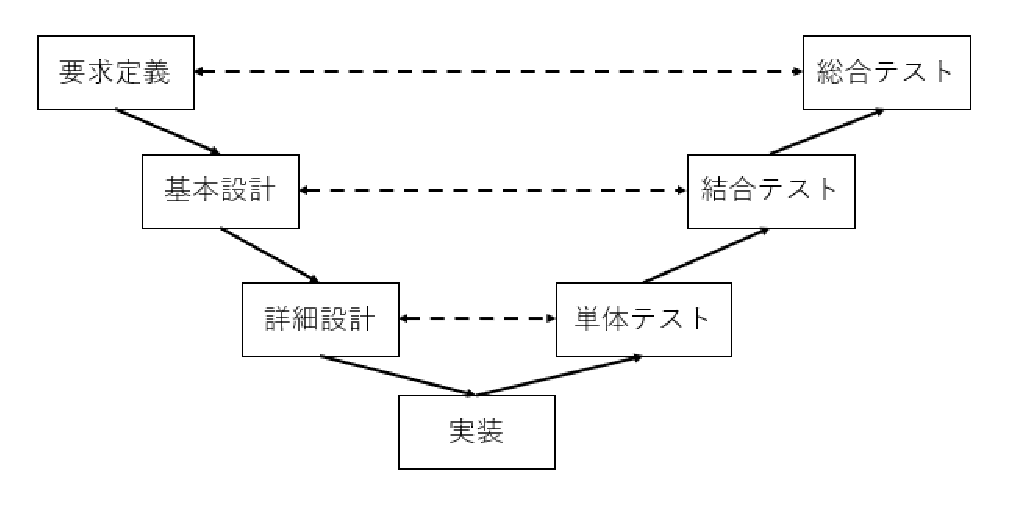
\includegraphics[height=60mm]{vmodel.eps}
	\caption{V字開発モデル}
        \label{fig:vmodel}
\end{center}
\end{figure}

%2章6節
\subsection{UML(Unified Modeling Language)}
UMLとは,オブジェクト指向分析,
設計においてシステムをモデル化する際の記法を規定した言語である.
UMLの用途は,プログラムを書く前に図で考えを整理すことや,
チーム開発において図でコミュニケーションをとること,
ユーザーや顧客と仕様を検討するなどの場合である\cite{uml}.

\subsection{ユースケース図}
ユースケース図とは,システムの仕様機能(ユースケース)と,外部環境(アクター)との関連を表す\cite{uml}.
一目でシステムの機能やシステム外部と内部の境界を理解することができるため,
ユーザーとクライアントとの意識統一を図ることが容易になる.
ユースケース図において,ユースケースはシステムの使用機能を楕円の中にユースケース名として記述する.
アクターは,機能を利用するユーザーや,システムが使用するハードウェア,外部システムを表現する.

\subsection{シーケンス図}
シーケンス図とは,オブジェクトの相互作用を表す相互作用図の一つで,
オブジェクト間のメッセージのやりとりを,時系列に沿って表現する\cite{uml}.

\subsection{クラス図}
クラス図とは,モデルの静的な構造を表し,システムの構造を表現できる\cite{uml}.
パッケージ単位の表現や,全体での表現,または,機能単位での表現など,様々な視点で作成することができる.
